\documentclass{article}
\usepackage{amsmath}
\usepackage{hyperref}
\usepackage{graphicx}
\usepackage{float}
\usepackage[top=2cm]{geometry}

\title{Deep Learning - Homework 1}
\author{99222 - Frederico Silva, 99326 - Sebastião Carvalho}
\date{\today}

\begin{document}

\maketitle

\tableofcontents

\section{Question 1}

Medical image classification with linear classifiers and neural networks.

\subsection{Question 1.1}

\subsubsection{Question 1.1 a)}

\paragraph{Answer} After running the code, the following plot was generated:
\begin{figure}[H]
    \centering
    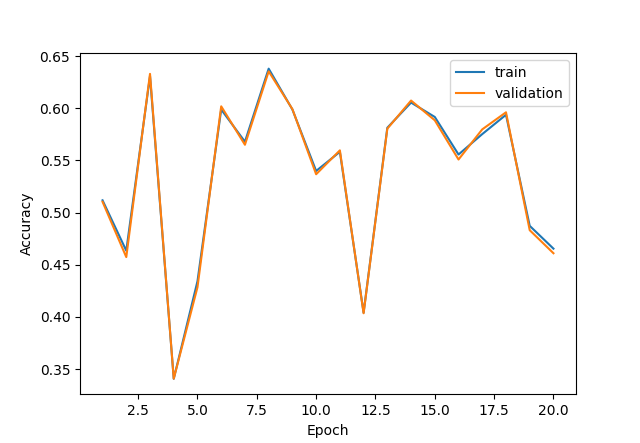
\includegraphics[width=0.8\textwidth]{"plots/1_1_a.png"}
    \caption{Classification of points using the function \( f \)}
    \label{1.1.a Plot}
\end{figure}

The final test accuracy was 0.3422.

\subsubsection{Question 1.1 b)}
\paragraph{Answer} After running the code, the following plots were generated, for learning rate $\eta = 0.01$ and $\eta = 0.001$, respectively:
\begin{figure}[H]
    \centering
    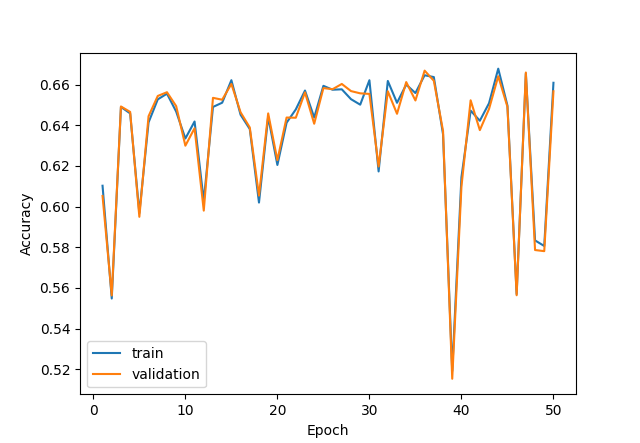
\includegraphics[width=0.8\textwidth]{"plots/1_1_b_001.png"}
    \caption{Classification of points using the function \( f \)}
    \label{1.1.b 0.01 Plot}
\end{figure}

\begin{figure}[H]
    \centering
    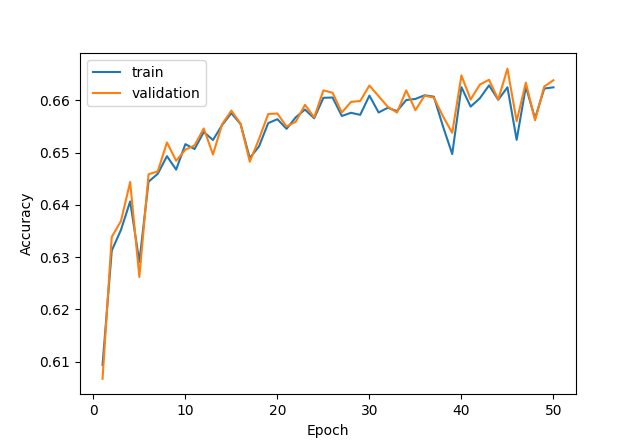
\includegraphics[width=0.8\textwidth]{"plots/1_1_b_0001.png"}
    \caption{Classification of points using the function \( f \)}
    \label{1.1.b 0.0001 Plot}
\end{figure}

The final test accuracy was 0.5784 and 0.5936 for $\eta = 0.01$ and $\eta = 0.001$ respectively.\\

\subsection{Question 1.2}

\subsubsection{Question 1.2 a)}
\subsubsection{Question 1.2 b)}

\section{Question 2}
Medical image classification with an autodiff toolkit.

\subsection{Question 2.1}

\subsection{Question 2.2}

\subsubsection{Question 2.2 a)}
\subsubsection{Question 2.2 b)}
\subsubsection{Question 2.2 c)}

\section{Question 3}

\subsection{Question 3.1}
\subsubsection{Question 3.1 a)}
\paragraph{Answer}

To demonstrate that the specified Boolean function cannot be computed by a single perceptron, let's consider a simple case where \( D = 2 \), \( A = -1 \), and \( B = 1 \). The function \( f \) is defined as:

\[
f(x) = 
\begin{cases} 
1 & \text{if } \sum_{i=1}^{D} x_i \in [-1, 1], \\
-1 & \text{otherwise}
\end{cases}
\]

In this setup:

\begin{itemize}
    \item For \( x = (+1, +1) \), the sum \( \sum x_i = 2 \). Since 2 is not in the range [-1, 1], \( f(x) = -1 \).
    \item For \( x = (-1, -1) \), the sum \( \sum x_i = -2 \). Since -2 is also not in the range [-1, 1], \( f(x) = -1 \).
    \item For \( x = (-1, +1) \) or \( x = (+1, -1) \), the sum \( \sum x_i = 0 \). This falls within the range [-1, 1], so \( f(x) = 1 \) for these inputs.
\end{itemize}

The visual representation of the points can be seen in Figure \ref{fig:points}. The red points represent the inputs that should be classified as \( +1 \) and the blue points represent the inputs that should be classified as \( -1 \).

The critical point here is that a single perceptron is fundamentally a linear classifier, which means it can only separate data points using a straight line in the feature space. However, in this example, there is no straight line that can separate these points accordingly in a 2D space to satisfy the function \( f \).

This example thus serves as a counter-example proving that the given function cannot generally be computed with a single perceptron, as it requires a non-linear decision boundary which a single perceptron cannot provide. 

\begin{figure}[H]
    \centering
    \includegraphics[width=0.8\textwidth]{"3a.png"}
    \caption{Classification of points using the function \( f \)}
    \label{3a Plot}
\end{figure}
\subsubsection{Question 3.1 b)}
\subsubsection{Question 3.1 c)}

\end{document}
